\section{Authentification du serveur et du client}

\subsection{Authentification du serveur} \label{Server's authentication}

L'authentification du serveur dans le protocole SSH se fait lors de l'échange de Diffie-Hellman (cf. §\ref{Échange d'un secret avec Diffie et Hellman}). On reprend ici les valeurs de l'échange: $A = g^a \: mod \: p$, $B = g^a \: mod \: p$ et $K = A^b \: mod \: p= B^a \: mod \: p=g^{ab} \: mod \: p$.

\paragraph{Client $\rightarrow$ Serveur}
Le client calcule $A$ et l'envoie au serveur. Ce dernier va alors directement calculer $B$ et $K$. Il va aussi calculer $H$, obtenu grâce à une fonction de hachage appliquée sur la concaténation:

\begin{itemize}
\item Des chaînes d'identification, celle du client que l'on notera $VC$ et celle du serveur que l'on notera $VS$ (cf. §\ref{S ID C/S});
\item Du message {\ttfamily SSH\verb|_|MSG\verb|_|KEXINIT}, celui envoyé par le client que l'on notera $IC$ ainsi que celui envoyé par le serveur que l'on notera $IS$ (cf. §\ref{KEXINIT});
\item De la clé publique du serveur, on la notera KS$_{pub}$
\item De $A$, envoyé par le client
\item De $B$, qu'il vient de calculer
\item De $K$, qu'il vient de calculer
\end{itemize}
Il faut noter que ces valeurs sont connues du client et du serveur, une fois que ce dernier a envoyé sa trame d'échange Diffie-Hellman. Le serveur chiffre ensuite H avec sa clé privée, que l'on notera KS$_{priv}$, ce qui donne $S$. Il envoie enfin au client KS$_{pub}$, $B$, et $S$.  \cite{lonvick_secure_2006} \label{ID C/S}

\paragraph{Serveur $\rightarrow$ Client}
Le client reçoit ces informations et va vérifier que la clé d'hôte publique appartient bien au serveur. Pour cela, il va vérifier la correspondance sur une base de données locale, ou avec un tiers de confiance, les serveurs PKI. Si aucune correspondance n'est trouvée, le client en est averti et peut choisir : de se déconnecter ou de poursuivre la connexion quand même. Cette méthode reste déconseillée car elle ne permet pas d'assurer réellement l'authentification du serveur. Si la connexion se poursuit quand même, le client calcule à son tour K et H (H est calculé de la même manière que décrite ci-dessus). Il peut alors déchiffrer S grâce à la clé publique de l'hôte, et retrouver le H que le serveur a calculé. Ce dernier doit être identique à celui calculé par le client.\cite{lonvick_secure_2006} \\

\begin{leftbar}
    \emph{Les PKI} (Public Key Infrastructure) sont des serveurs permettant à des clients d'obtenir la clé publique d'une machine de manière sécurisée, en étant certain que la clé donnée correspond bien à la machine voulue. La fiabilité de ces serveurs reposent sur une chaîne de confiance avec à la base un serveur que l'on sait \og vraiment fiable \fg \cite{perlman_overview_1999}
\end{leftbar}

\begin{figure}[H]
    \centering
    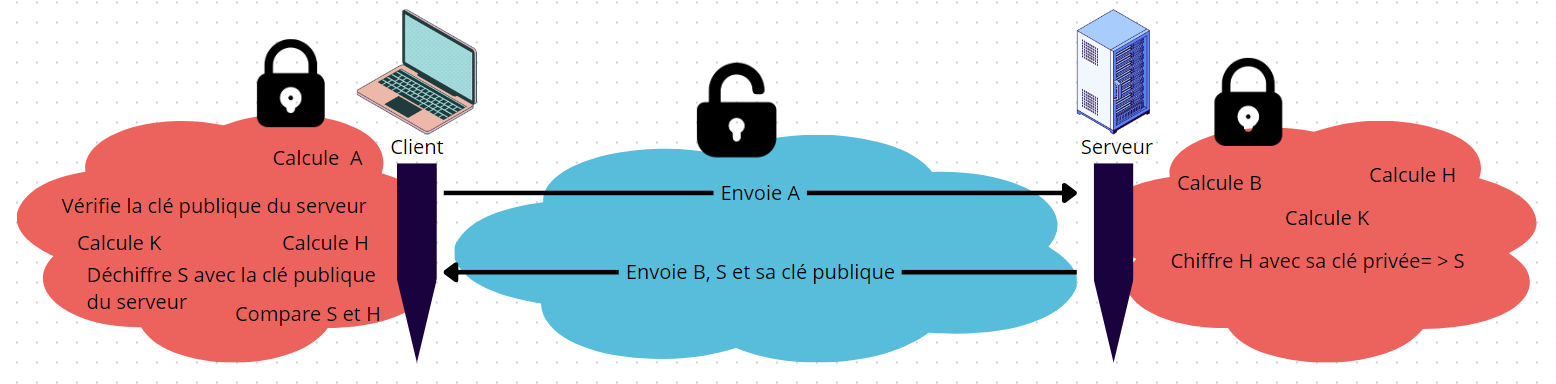
\includegraphics[width=1\linewidth]{images/Authentification serveur.png}
    \caption{Authentification du serveur. Source: \cite{cadegros_authentification_2023-1}}
\end{figure}

Une fois l'échange de clé terminé, le message {\ttfamily SSH\verb|_|MSG\verb|_|NEWKEYS} est envoyé par les deux parties et signale qu'à partir de ce message, les algorithmes utilisés et les clés de chiffrement utilisées seront ceux qu'ils viennent de définir. \cite{lonvick_secure_2006}. C'est la fin de la hand-shake énoncée §\ref{handshake}.

\subsection{Authentification du client}

Une fois l'hôte identifié, le client envoie une demande de service, c'est à dire une demande d'activation de la couche d'authentification ou de la couche connexion. La demande de ce dernier service est rejetée par le serveur si le client ne s'est pas authentifié avant, les machines se déconnectent alors. Le client doit donc d'abord s'authentifier \cite{hajjeh_ibrahim_protocole_2006}. Pour que ce dernier puisse le faire, 4 méthodes s'offrent à lui :

\paragraph{Méthode \textit{none}}
Cette méthode ne requiert aucune authentification auprès du serveur, n'importe quel client possédant l'adresse IP et le nom d'utilisateur du serveur peut s'y connecter. Il est évidemment fortement recommandé de ne pas utiliser cette technique.\cite{lonvick_secure_2006}

\paragraph{Méthode \textit{password}}
Le password est une chaîne de caractères connue du serveur. Lors de la connexion du client au serveur, cette chaîne lui est demandée. Elle est transmise en clair dans un paquet au serveur, cependant, le paquet reste crypté. Une fois le password récupéré par le serveur, il est vérifié selon les méthodes de l'OS installé sur le serveur et autorise la connexion au serveur.\cite{lonvick_secure_2006}

\paragraph{Méthode \textit{publickey}}
Cette méthode est la plus courante et doit être obligatoirement activée, elle est la plus recommandée. Une \textit{passphrase} est générée par le serveur et transmise en clair via les échanges cryptés au client. Cette \textit{passphrase} sera cryptée par un chiffrement asymétrique, le client cryptant avec sa clé privée l'information. Elle est transmise désormais cryptée au serveur via les échanges cryptés. Le serveur possède les clés publiques des clients autorisés à se connecter. Il déchiffre donc l'information avec la clé publique du client. Si l'information décryptée et la \textit{passphrase} concordent, le client est autorisé à se connecter. \cite{lonvick_secure_2006}

\begin{figure}[H]
    \centering
    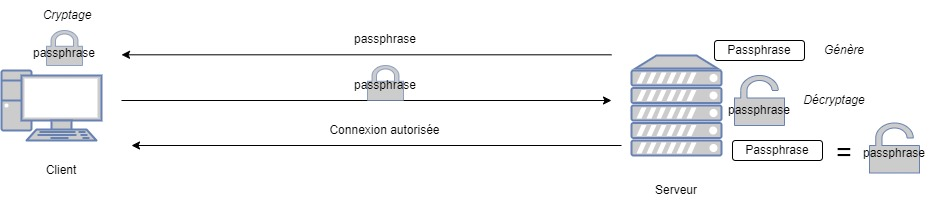
\includegraphics[width=1\linewidth]{images/PublicKey_Aiuthentification_Method.jpg}
    \caption{Authentification du client auprès du serveur : Méthode \textbf{publikey} - Source : \cite{cadegros_authentification_2023}}
    \label{fig:enter-label}
\end{figure}

\paragraph{Méthode \textit{hotbased}}
Cette méthode d'authentification est basée sur l'hébergeur du client, elle permet à l'ensemble des clients de l'hébergeur d'obtenir un accès distant au serveur, il est donc indispensable de prendre des précautions lors de la mise en place de cette méthode qui pourrait donner des privilèges à n'importe quel utilisateur. Lorsque le client se connecte, le serveur vérifie que le nom d'hôte est présent dans son fichier \textit{rhosts}, et vérifie si le programme demandé est autorisé en vérifiant si son port d'écoute est compris entre 1 et 1023. En effet, ces ports d'écoute sont dits sûrs puisque activables seulement par l'administrateur.\cite{hajjeh_ibrahim_protocole_2006}

\subsection{Authentification par RSA}

La méthode d'authentification par publickey du client ou celle du serveur nécessite une utilisation d'une méthode cryptographique asymétrique. Pour cela, nous pouvons utiliser le RSA. Commençons par introduire le cryptage RSA au sens global.

\subsubsection{Groupe multiplicatif}

Considérons le groupe multiplicatif $(\frac{\mathbb{Z}}{n\mathbb{Z}})^{\times}$ (cf. §\ref{Notion de groupe}) soit l'ensemble des éléments inversibles du groupe $(\frac{\mathbb{Z}}{n\mathbb{Z}})$, considérons $k$ un élément de $(\frac{\mathbb{Z}}{n\mathbb{Z}})^{\times}$, montrons qu'alors $k$ et $n$ sont premiers entre eux.\\

Si $k \in (\frac{\mathbb{Z}}{n\mathbb{Z}})^{\times}$, alors il existe un entier $l \in (\frac{\mathbb{Z}}{n\mathbb{Z}})^{\times}$ tel que $l$ soit l'inverse de $k$ donc $k\times l = 1$, il existe donc $m \in \mathbb{Z}$ tel que $kl - 1 = mn \Leftrightarrow kl-mn=1$, d'après le théorème de Bezout (cf. §\ref{Notion de groupe}), $n$ et $k$ sont premiers.\\

Ainsi, le cardinal de $(\frac{\mathbb{Z}}{n\mathbb{Z}})^{\times}$ correspond au nombre d'éléments $k$ tels que $k$ et $n$ soient premiers entre eux, soit la fonction d'Euler de $n$ notée $\varphi(n)$.\cite{rostam_groupe_nodate}\\

\subsubsection{Génération de clés RSA} \label{Gen RSA key}
Prenons deux nombres premiers distincts $p$ et $q$ tels que $n=pq$, le cardinal du groupe $(\frac{\mathbb{Z}}{n\mathbb{Z}})^{\times}$ est donc $\varphi(n)=(p-1)(q-1)$ \cite{cormen_algorithmes_2013}. On génère un entier $e$ premier avec $\varphi(n)$ et son inverse $d$,

\[d\times e = 1 \: mod \: (\varphi(n))\]

Nous pouvons utiliser l'algorithme d'Euclide étendu pour déterminer l'inverse modulaire de $e$ noté $d$ \cite{cormen_algorithmes_2013}.

\begin{algorithm}[H]
\caption{Algorithme d'Euclide étendu pour trouver l'inverse}
\KwData{Valeurs de $x$ et $\varphi(n)$}
\KwResult{Inverse de $x \: mod \: \varphi(n)$}

$a \gets$ \text{valeur de } $x$\;
$b \gets$ \text{valeur de } $\varphi(n)$\;
$u1 \gets 1$, $v1 \gets 0$\;
$u2 \gets 0$, $v2 \gets 1$\;

\While{$b \neq 0$}{
    $quotient \gets a \div b$\;
    $reste \gets a \mod b$\;
    $u \gets u1 - quotient \times u2$\;
    $v \gets v1 - quotient \times v2$\;

    \tcp{Mise à jour des variables pour la prochaine itération}
    $a \gets b$\;
    $b \gets reste$\;
    $u1 \gets u2$\;
    $v1 \gets v2$\;
    $u2 \gets u$\;
    $v2 \gets v$\;
}

\If{$a = 1$}{
    \tcp{À la fin de la boucle, $u1$ est l'inverse de $a \: mod \: \varphi(n)$}
    $inverse \gets u1 \mod b$\;
    \textbf{Retouner} $inverse$\;
}
\Else{
    \textbf{Retourner} "L'inverse n'existe pas, car", $a$, "et", $b$, "ne sont pas premiers entre eux."\;
}

\end{algorithm}

Nous obtenons deux couples $Pr = (e,n)$ $Pu = (e,d)$, les clés respectivement privées et publiques de notre système.

\subsubsection{Fonctions de cryptage RSA}
La fonction de cryptage de la cryptographie RSA est la suivante, avec $x$ l'élément à chiffrer \cite{cormen_algorithmes_2013} :

\[ F(x) = x^y \: mod \: n\]

$y$ correspond à $d$ ou $e$ en fonction de la clé de cryptage utilisée. L'élément à chiffrer peut-être un nombre représentant des données comme du texte converti en binaire avec le langage ASCII. Montrons désormais que cette fonction de cryptage peut permettre de décrypter une information cryptée avec la première clé à l'aide de la seconde. Pour cela, démontrons que les fonctions suivantes sont l'inverse l'une de l'autre :

\[ Fpu(x) = x^d \: mod \: n\]
\[ Fpr(x) = x^e \: mod \: n\]

Prenons un élément $x$ à crypter, en le cryptant avec la fonction $Fpu(x)$ nous obtenons $x^d \: mod \: n$. Désormais passons ce nombre dans la seconde fonction de cryptage, nous obtenons $x^{de} \: mod \: n$, montrons que ce nombre est égal à $c \: mod \: n$. Rappelons que $n=pq$, d'après le petit théorème de Fermat, $(c \: mod \: p)^{p-1} \: mod \: p = 1$ or $e$ et $d$ sont des inverses multiplicatifs modulo $\varphi(n)$. Soit pour un entier $h$, on peut écrire $ed = 1 + h(p-1)(q-1)$. Si $t \: mod \: p \neq 0$ alors :


\[\Leftrightarrow x^{ed} \: mod \: p = (x \: mod \: p)^{ed} \: mod \: p\]
\[\Leftrightarrow x^{ed} \: mod \: p = (x \: mod \: p)^{1+h(p-1)(q-1)} \: mod \: p\]
\[\Leftrightarrow x^{ed} \: mod \: p = ((x \: mod \: p).((x \: mod \: p)^{p-1} \: mod \: p)^{h(q-1)}) \: mod \: p\]
\[\Leftrightarrow x^{ed} \: mod \: p = (x \: mod \: p).(1^{h(q-1)} \: mod \: p)\]
\[\Leftrightarrow x^{ed} \: mod \: p = x \: mod \: p\]

Si $x \: mod \: p = 0$ alors $x^{ed} \: mod \: p = 0$. De même, on peut montrer Si $x \: mod \: q = 0$ alors $x^{ed} \: mod \: q = 0$ et si $x \: mod \: q \neq 0$ alors $x^{ed} \: mod \: q = x \: mod \: q$. De plus, si $x^{ed} \: mod \: p = x \: mod \: p$ et $x^{ed} \: mod \: q = x \: mod \: q$ alors $x^{ed} \: mod \: pq = x \: mod \: pq$, sachant que $n=pq$ on obtient : 

\[x^{ed} \: mod \: n = x \: mod \: n\]

Les fonctions de cryptage par les clés publiques et privées sont donc des fonctions inverses, elles permettent de crypter ou décrypter l'information cryptée par une autre clé \cite{cormen_algorithmes_2013}.

\subsubsection{Problème de factorisation des grands entiers}

La sécurité du chiffrement RSA, repose sur le principe de factorisation du modulo $n$. En effet, si un attaquant est en possession de $n$, et s'il est capable de le factoriser en deux nombres premiers $p$ et $q$ alors, en faisant les opérations du §\ref{Gen RSA key}, il est en mesure d'obtenir les clés publique et privée.\cite{hostalot_attaque_nodate}\\

L'algorithme NFS est l'algorithme le plus rapide connu à ce jour pour résoudre ce problème \cite{hostalot_attaque_nodate}. Il repose sur le principe de la congruence carrée, en recherchant des paires d'entiers $x$ et $y$ telles que


\[x^2 = y^2 \: mod \: n\]

Ceci avec pour objectif de trouver un facteur de $n$ en calculant $pgcd(x-1,n)$ et $pgcd(x+y,n)$. \cite{bouvier_algorithmes_2015}. Les étapes de l'algorithme sont les suivantes :

\begin{enumerate}
    \item \textbf{Sélection ploynomiale :} Pour commencer, nous devons choisir deux paires de polynômes irréductibles à coefficients entiers : $f_0$ et $f_1$ premiers entre eux et possédant une racine commune notée $m \: mod \: n$.\cite{bouvier_algorithmes_2015}

    \item \textbf{Collecte des relations :} Cette étape consiste à identifier deux entiers $Res(a-bx, f_0)$ et $Res(a+bx, f_1)$ des entiers résultants de chaque polynôme, dans un espace indexé par les entiers $a$ et $b$. De sorte que leurs plus grands facteurs premiers soient plus petits à deux entiers fixés (deux bornes). Cette étape étant coûteuse en ressource, on peut se permettre d'utiliser de grandes bornes. \cite{hostalot_attaque_nodate}. Des relations obtenues, il en est déduit plusieurs sous ensembles. 

    \item \textbf{Algèbre linéaire} De ces relations et sous-ensembles est obtenu un système linéaire.\cite{hostalot_attaque_nodate}

    \item \textbf{calculs finaux :} Des calculs finaux faisant appel à des techniques d’arithmétique multiprécision sur des entiers de très grandes tailles permettent d'obtenir les nombres $p$ et $q$. \cite{hostalot_attaque_nodate}

\end{enumerate}

Lors de ces étapes, la recherche des relations ainsi que l'algèbre linéaire sont très coûteuses en ressources. Par exemple, pour un modulo de $829 bits$, la recherche de relation pour un processeur Intel Xeon 6130 (2.1 GHz) est de 794 années-cœurs \cite{hostalot_attaque_nodate} et la recherche totale des entiers $p$ et $q$ 953 années-cœurs \cite{hostalot_attaque_nodate}. La factorisation d'un modulo de 1 024 bits devrait être bien plus longue, avec une durée de 500 000 années-cœurs. \cite{hostalot_attaque_nodate}.\\

Ceci met en évidence la nécessité d'utiliser des modulos de grandes tailles pour garantir la sécurité des échanges. Ceci est d'autant plus important que les clés RSA sont très peu renouvelées.

\subsubsection{RSA et SSH}
Ainsi, nous privilégierons pour garantir la sécurité de l'authentification une clé RSA-2048 composée d'un modulo de 2048 bits. Il est nécessaire que le client ait transmis au serveur en amont sa clé publique. Ceci peut se dérouler lors d'une précédente session, directement sur le serveur, ou via un service externe comme dans le cas de GitHub qui propose de rentrer sa clé RSA publique directement dans les paramètres de son compte. Dans le cas de l'authentification du serveur, la clé publique est transmise durant l'échange de clé de Diffie-Hellman (cf. §\ref{Server's authentication}).